
\documentclass{article}

%% Packages for French writing
\usepackage[french]{babel}
\usepackage[utf8]{inputenc}
\usepackage[T1]{fontenc}
\usepackage{layout}

%% Packages for Math symbols
\usepackage[fleqn]{amsmath}
\usepackage{amssymb}
\usepackage{mathrsfs}

%% Packages for figures insertion
\usepackage{graphicx}
\usepackage{wrapfig}
\usepackage{framed}
\usepackage{float}

%% Package for document margin editing
\usepackage[top=2cm, bottom=2cm, left=2cm, right=2cm]{geometry}

%% Package for source code insertion
\usepackage{listings}
\usepackage{xcolor}
\definecolor{grey}{rgb}{0.97, 0.97, 0.97}
\definecolor{darkred}{rgb}{0.42, 0, 0}
\definecolor{darkblue}{rgb}{0, 0, 0.42}
\definecolor{darkgrey}{rgb}{0.22, 0.22, 0.82}
\definecolor{green}{HTML}{088A08}
\lstset{
  basicstyle=\small\sffamily\footnotesize,
  captionpos=b,
  numbers=left,
  numberstyle=\tiny,
  tabsize=4,
  frame=trBL,
  backgroundcolor=\color{grey},
  commentstyle=\color{green},
  keywordstyle=\color{darkblue}\bf,
  identifierstyle=\color{darkgrey},
  stringstyle=\color{darkred}
}

\setlength\parindent{0pt}
\setlength\parskip{3pt}
\title{ARCHI2 - Compte-rendu du TME1}
\author{Nicolas Phan}
\date{pour le 16 Février 2018}
\begin{document}
\pagestyle{headings}
\maketitle
\tableofcontents
\newpage

%==================================================================================================
%=========================  Introduction  =========================================================
%==================================================================================================

%----------------- Objectif -----------------------------------------------------------------------

\section{Automate du composant PibusSimpleRam}

\begin{figure}[H]
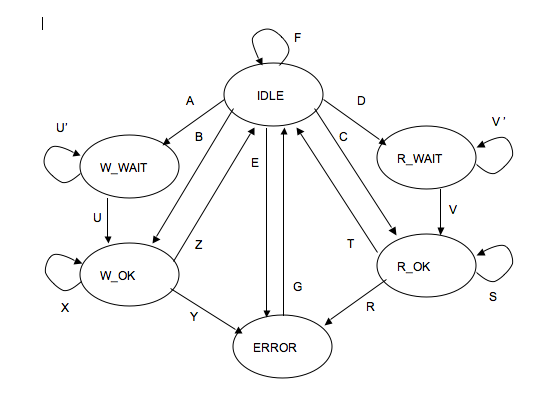
\includegraphics[width=0.75\textwidth]{pics/mae_ram.png}
\centering
\caption{Graphe de la MAE du composant RAM}
\label{mae_ram}
\end{figure}

\begin{table}[H]
\centering
\begingroup
\setlength{\tabcolsep}{5pt}
\renewcommand{\arraystretch}{1.1}
\begin{tabular}{| l | p{15cm} |}
\hline
Etat    & Signification \\
\hline
\tt{IDLE}    & La RAM est inactive, elle n'est la cible d'aucune transaction \\
\hline
\tt{W\_WAIT}   & Une transaction d'écriture dans le composant RAM est en cours,
        l'automate attend que la RAM soit disponible. \\
\hline
\tt{W\_OK}     & Une transaction d'écriture dans le composant RAM est en cours,
        la RAM effectue l'écriture. \\
\hline
\tt{R\_WAIT}   & Une transaction de lecture dans le composant RAM est en cours,
        l'automate attend que la RAM doit disponible \\
\hline
\tt{R\_OK}     & Une transaction de lecture dans le composant RAM est en cours,
        la RAM a effectue la lecture \\
\hline
\tt{ERROR}   & Une erreur s'est produite \\
\hline
\end{tabular}
\caption{Description des états de la MAE}
\endgroup
\end{table}

\subsection{Question C1}

\begin{table}[H]
\centering
\begingroup
\setlength{\tabcolsep}{5pt}
\renewcommand{\arraystretch}{1.1}
\begin{tabular}{ | l | l | l | }
\hline
Nom    &   Transition  &    Explication \\
\hline
\texttt{A}  &   \tt{SEL.ADR\_OK.$\overline{\tt{READ}}$.DELAY                     } &
Une requête d'écriture a été recue, la RAM est latente donc l'automate attend. \\
\texttt{B}  &   \tt{SEL.ADR\_OK.$\overline{\tt{READ}}$.$\overline{\tt{DELAY}}$        } &
Une requête d'écriture a été recue, l'écriture s'effectue. \\
\texttt{C}  &   \tt{SEL.ADR\_OK.READ.$\overline{\tt{DELAY}}$                     } &
idem en lecture \\
\texttt{D}  &   \tt{SEL.ADR\_OK.READ.DELAY                                  } &
idem en lecture \\
\texttt{E}  &   \tt{SEL.$\overline{\tt{ADR\_OK}}$                                } &
Le composant RAM est la cible d'une transaction comportant une adresse illégale. \\
\texttt{F}  &   \tt{$\overline{\tt{SEL}}$                                        } &
Le composant RAM n'est pas sélectionné pour une transaction, il reste inactif. \\
\texttt{G}  &   \tt{1                                                       } &
Il n'y a qu'une seule transition sortant de ERROR, elle est donc inconditionnelle. \\
\hline
\texttt{U}  &   \tt{$\overline{\tt{GO}}$                                         } &
La RAM est latente, l'automate reste en état d'attente. \\
\texttt{U'} &   \tt{GO                                                      } &
La RAM effectue l'écriture, le composant est à l'état READY \\
\hline
\texttt{V}  &   \tt{$\overline{\tt{GO}}$                                         } &
idem en lecture \\
\texttt{V'} &   \tt{GO                                                      } &
idem en lecture \\
\hline
\texttt{X}  &   \tt{SEL.ADR\_OK.$\overline{\tt{READ}}$                           } &
Le composant RAM est toujours sélectionné, ses entrées n'ont pas changé \\
\texttt{Y}  &   \tt{SEL.($\overline{\tt{ADR\_OK}}$ + READ)                       } &
Le composant RAM est toujours sélectionné mais ses entrées ont été corrompues \\
\texttt{Z}  &   \tt{$\overline{\tt{SEL}}$                                        } &
La transaction se termine, le composant RAM n'est plus sélectionnée \\
\hline
\texttt{R}  &   \tt{SEL.($\overline{\tt{ADR\_OK}}$ + $\overline{\tt{READ}}$)          } &
idem en lecture \\
\texttt{S}  &   \tt{SEL.ADR\_OK.READ                                        } &
idem en lecture \\
\texttt{T}  &   \tt{$\overline{\tt{SEL}}$                                        } &
idem en lecture \\
\hline
\end{tabular}
\caption{Fonctions de transition de la MAE de SimpleRam}
\endgroup
\end{table}

       

\subsection{Question C2}

\begin{table}[H]
\centering
\begingroup
\setlength{\tabcolsep}{5pt}
\renewcommand{\arraystretch}{1.1}
\begin{tabular}{| l | l | l | l | l |}
\hline
                    & \tt{ACK\_EN}      & \tt{ACK\_VALUE}   & \tt{DT\_EN} & \tt{MEM\_CMD}   \\
\hline
\tt{IDLE}           & \tt{0}            & \tt{WAIT}         & \tt{0}      & \tt{NOPE}         \\
\tt{R\_WAIT}        & \tt{1}            & \tt{WAIT}         & \tt{0}      & \tt{READ}         \\
\tt{R\_OK}          & \tt{1}            & \tt{READY}        & \tt{0}      & \tt{READ}         \\
\tt{W\_WAIT}        & \tt{1}            & \tt{WAIT}         & \tt{1}      & \tt{WRITE}        \\
\tt{W\_OK}          & \tt{1}            & \tt{READY}        & \tt{1}      & \tt{WRITE}        \\
\tt{ERROR}          & \tt{1}            & \tt{ERROR}        & \tt{0}      & \tt{NOPE}         \\
\hline
\end{tabular}
\caption{Valeurs des signaux de sortie de la MAE de SimpleRam}
\endgroup
\end{table}







\section{Automate du composant PibusSimpleMaster}

\begin{figure}[H]
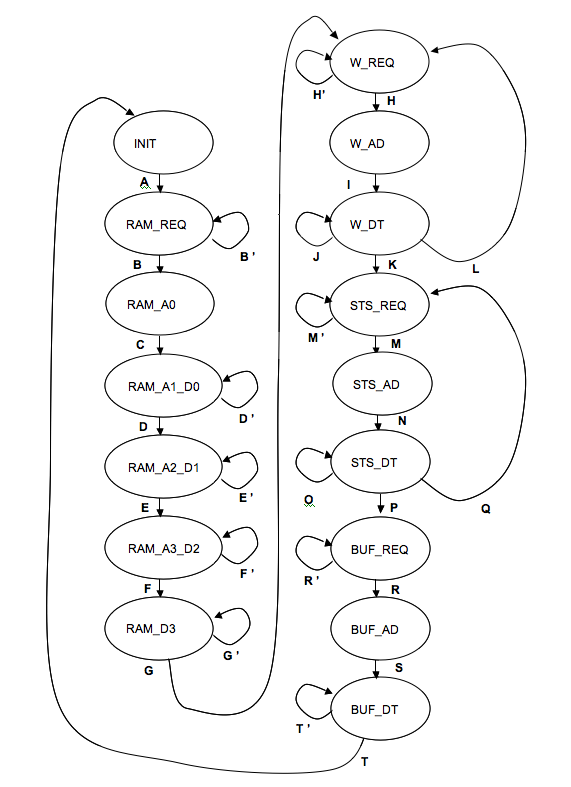
\includegraphics[width=0.75\textwidth]{pics/mae_master.png}
\centering
\caption{Graphe de la MAE du composant Master}
\label{mae_ram}
\end{figure}

\begin{table}[H]
\centering
\begingroup
\setlength{\tabcolsep}{5pt}
\renewcommand{\arraystretch}{1.1}
\begin{tabular}{ | l | p{15cm} | }
\hline
Etat    & Signification \\
\hline

\tt{INIT}    &
Etat initial \\
\hline

\tt{RAMREQ}  &
Le maitre demande l'accès au bus pour y effectuer une transaction rafale
de lecture de 4 mots dans la RAM. \\
\hline

\tt{RAMA0}   &
Le maitre vient d'obtenir le bus, il fournit la première adresse \\
\hline

\tt{RAMA1D0} &
Le maitre envoie une adresse qui n'est pas la première de la transaction :
il effectue un transfert rafale. \\
\hline

\tt{RAMA2D1} &
Idem, ici le maitre envoie la troisème adresse de la rafale \\
\hline

\tt{RAMA3D2} &
Idem, ici le maitre envoie la quatrième adresse de la rafale \\
\hline

\tt{RAMD3}   &
Le maitre attend la dernière réponse de la RAM. \\
\hline

\tt{WREQ}    &
Le maitre demande l'accès au bus pour y effectuer une transaction d'écriture
dans le registre DISPLAY du composant TTY dans le but d'afficher un caractère
à l'écran. \\
\hline

\tt{WAD} &
Le maitre vient d'obtenir le bus il fournit sa commande. \\
\hline

\tt{WDT} &
Le maitre attend la réponse de la cible \\
\hline

\tt{STSREQ}  &
Le maitre demande l'accès au bus pour une transaction de lecture du registre
STATUS du périphérique TTY afin de déterminer si un caractère a été entré au clavier. \\
\hline

\tt{STSAD}   &
Le maitre vient d'obtenir le bus il fournit sa commande. \\
\hline

\tt{STSDT}   &
Le maitre attend la réponse de la cible \\
\hline

\tt{BUFREQ}  &
Le maitre demande l'accès au bus pour une transaction de lecture du registre
KEYBUF du TTY afin de connaitre le caractère entré au clavier par l'utilisateur. \\
\hline

\tt{BUFAD}   &
Le maitre vient d'obtenir le bus il fournit sa commande. \\
\hline

\tt{BUFDT}   &
Le maitre attend la réponse de la cible \\
\hline

\end{tabular}
\endgroup
\caption{Description des etats de l'automate}
\end{table}


\subsection{Question D1}

\begin{table}[H]
\centering
\begingroup
\setlength{\tabcolsep}{5pt}
\renewcommand{\arraystretch}{1.1}
\begin{tabular}{ | l | l | p{15cm} |}
\hline
Nom    &   Transition  & Description \\
\hline
\tt{A}  & \tt{1} &
Une seule transition sort de l'etat INIT, elle est donc inconditionnelle \\
\tt{B'} & \tt{$\overline{\tt{GNT}}$} &
Le composant master demande le BUS tant qu'il ne l'a pas obtenu. \\
\tt{B}  & \tt{GNT} &
Le maitre a obtenu le bus, il va envoyer sa première commande \\
\hline
\tt{C}  & \tt{1} &
D'après le protocole PIBUS, lors d'une transaction rafale, la première commande
est toujours enregistrée par la cible, donc le maitre passe inconditionnellement
à la deuxième commande une fois que la première est envoyée. \\
\tt{D'} & \tt{RDY} &
Tant que la cible n'a pas acquitté, le maitre continue d'envoyer sa commande. \\
\tt{D}  & \tt{$\overline{\tt{RDY}}$} &
Le maitre a eu l'acquittement de la cible, il passe à la commande suivante. \\
\tt{E}  & \tt{RDY} &
idem \\
\tt{E'} & \tt{$\overline{\tt{RDY}}$} &
idem \\
\tt{F}  & \tt{RDY} &
Le maitre a bien recu l'avant-dernière réposne, il ne lui reste plus
qu'à attendre la dernière réponse. \\
\tt{F'} & \tt{$\overline{\tt{RDY}}$} &
idem \\
\tt{G}  & \tt{RDY} &
Le maitre a recu la dernière réponse, la transaction se termine,
il passe à la transaction suivante. \\
\tt{G'} & \tt{$\overline{\tt{RDY}}$} &
Le maitre reste en état d'attente tant qu'il n'a pas recu la dernière réponse. \\
\hline
\tt{H'} & \tt{$\overline{\tt{GNT}}$} &
même situation que B' \\
\tt{H}  & \tt{GNT} &
même situation que B \\
\tt{I}  & \tt{1} &
Le maitre a envoyé sa commande, il va attendre la réponse \\
\tt{J}  & \tt{$\overline{\tt{RDY}}$} &
Le maitre attend sa réponse de la cible tant qu'il ne l'a pas eue. \\
\tt{K}  & \tt{RDY.LAST} &
Le maitre a obtenu une réponse de la cible (RDY, on ne traite pas les cas d'erreur)
et le caractère envoyé était le dernier, le maitre passe à l'étape suivante. \\
\tt{L}  & \tt{RDY.$\overline{\tt{LAST}}$} &
Idem, sauf qu'il ne s'agit pas du dernier caractère, le maitre engage une nouvelle transaction
pour envoyer le caractère suivant. \\
\hline
\tt{M'} & \tt{$\overline{\tt{GNT}}$} &
même situation que H' \\
\tt{M}  & \tt{GNT} &
même situation que H \\
\tt{N}  & \tt{1} &
même situation que I \\
\tt{O}  & \tt{$\overline{\tt{RDY}}$} &
même situation que J \\
\tt{P}  & \tt{RDY.$\overline{\tt{NUL}}$} &
Le maitre a obtenu le contenu du registre STATUS, et ce-dernier indique qu'un caractère
a été entré. \\
\tt{Q}  & \tt{RDY.NUL} &
Aucun caractère n'a été entré, le maitre continue la lecture en boucle de STATUS. \\
\hline
\tt{R'} & \tt{$\overline{\tt{GNT}}$} &
même chose que H' \\
\tt{R}  & \tt{GNT} &
même chose que H \\
\tt{S}  & \tt{1} &
même chose que I \\
\tt{T'} & \tt{$\overline{\tt{RDY}}$} &
La transaction est terminée \\
\tt{T}  & \tt{RDY} &
même chose que J \\
\hline
\end{tabular}
\endgroup
\caption{Fonctions de transitions de la MAE de SimpleMaster}
\end{table}

\subsection{Question D2}

\begin{table}[H]
\centering
\begingroup
\setlength{\tabcolsep}{5pt}
\renewcommand{\arraystretch}{1.1}
\begin{tabular}{|l|l|l|l|l|l|l|}
\hline
                  & \tt{REQ}       & \tt{CMD\_EN}   & \tt{ADR\_VALUE}         & \tt{READ\_VALUE}   & \tt{LOCK\_VAL} & \tt{DT\_EN}    \\
\hline
\tt{INIT}         & \tt{0}         & \tt{0}         & \tt{X}                  & \tt{X}             & \tt{X}         & \tt{0}         \\
\tt{RAM\_REQ}     & \tt{1}         & \tt{0}         & \tt{X}                  & \tt{X}             & \tt{X}         & \tt{0}         \\
\tt{RAM\_A0}      & \tt{0}         & \tt{1}         & \tt{ram\_base}          & \tt{1}             & \tt{1}         & \tt{0}         \\
\tt{RAM\_A1D0}    & \tt{0}         & \tt{1}         & \tt{ram\_base + 4}      & \tt{1}             & \tt{1}         & \tt{0}         \\
\tt{RAM\_A2D1}    & \tt{0}         & \tt{1}         & \tt{ram\_base + 8}      & \tt{1}             & \tt{1}         & \tt{0}         \\
\tt{RAM\_A3D2}    & \tt{0}         & \tt{1}         & \tt{ram\_base + 12}     & \tt{1}             & \tt{1}         & \tt{0}         \\
\tt{RAM\_D3}      & \tt{0}         & \tt{0}         & \tt{X}                  & \tt{X}             & \tt{0}         & \tt{0}         \\
\tt{W\_REQ}       & \tt{1}         & \tt{0}         & \tt{X}                  & \tt{X}             & \tt{X}         & \tt{0}         \\
\tt{W\_AD}        & \tt{0}         & \tt{1}         & \tt{seg\_tty\_base}     & \tt{0}             & \tt{0}         & \tt{0}         \\
\tt{W\_DT}        & \tt{0}         & \tt{0}         & \tt{seg\_tty\_base}     & \tt{0}             & \tt{0}         & \tt{1}         \\
\tt{STS\_REQ}     & \tt{1}         & \tt{0}         & \tt{X}                  & \tt{X}             & \tt{X}         & \tt{0}         \\
\tt{STS\_AD}      & \tt{0}         & \tt{1}         & \tt{seg\_tty\_base + 4} & \tt{1}             & \tt{0}         & \tt{0}         \\
\tt{STS\_DT}      & \tt{0}         & \tt{0}         & \tt{seg\_tty\_base + 4} & \tt{1}             & \tt{0}         & \tt{0}         \\
\tt{BUF\_REQ}     & \tt{1}         & \tt{0}         & \tt{X}                  & \tt{X}             & \tt{X}         & \tt{0}         \\
\tt{BUF\_AD}      & \tt{0}         & \tt{1}         & \tt{seg\_tty\_base + 8} & \tt{1}             & \tt{0}         & \tt{0}         \\
\tt{BUF\_DT}      & \tt{0}         & \tt{0}         & \tt{X}                  & \tt{X}             & \tt{X}         & \tt{0}         \\
\hline
\end{tabular}
\endgroup
\caption{Valeurs de sortie de la MAE de SimpleMaster}
\end{table}


\section{Automate du composant PibusSegBcu}

\begin{figure}[H]
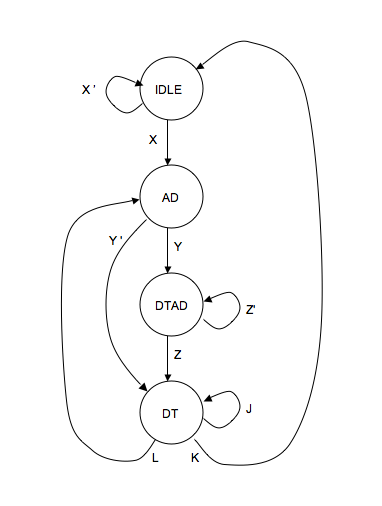
\includegraphics[width=0.5\textwidth]{pics/mae_bus.png}
\centering
\caption{Graphe de la MAE du composant BCU}
\label{mae_ram}
\end{figure}

\begin{table}[H]
\centering
\begingroup
\setlength{\tabcolsep}{5pt}
\renewcommand{\arraystretch}{1.1}
\begin{tabular}{ | l | p{15cm} |}
\hline
Etat    & Description \\
\hline
IDLE    &
Le BCU est libre et attend une requête,
le BCU et le maitre sont inactifs \\
\hline
AD      &
Le bus vient d'être alloué au maitre, la première commande est envoyée \\
\hline
DTAD    &
Le bus est alloué à un maitre, il envoie une commande qui n'est pas la première
de la transaction en cours (le maitre est en train d'effectuer une transaction rafale) \\
\hline
DT      &
Le maitre attend la dernière réponse de la cible, le bus ne lui est plus alloué \\
\hline
\end{tabular}
\endgroup
\caption{Description des etats de l'automate}
\end{table}


\subsection{Question E1}

\begin{table}[H]
\centering
\begingroup
\setlength{\tabcolsep}{5pt}
\renewcommand{\arraystretch}{1.1}
\begin{tabular}{ | l | l | p{10cm} |}
\hline
Nom    &   Transition  \\
\hline
\tt{X}      & \tt{$\overline{\tt{REQ}}$} &
Tant que l'unique maitre ne demande pas le bus, le BCU reste inactif. \\
\hline

\tt{X}      & \tt{REQ} &
Le maitre a demandé le BCU, comme il est le seul maitre ici, il obtient le bus. \\
\hline

\tt{Y}      & \tt{LOCK} &
Il s'agit d'une transaction rafale \\
\hline

\tt{Y'}      & \tt{$\overline{\tt{LOCK}}$} &
IL ne s'agit pas d'une transaction rafale, l'automate va simplement attendre
la réponse de la cible. \\
\hline

\tt{Z'}      & \tt{LOCK + $\overline{\tt{(ACK != WAIT)}}$} &
Tant que le maitre n'a pas envoyé toutes ses commandes ou n'a pas recu
d'acquittement à celles-ci (excepté pour la dernière), la rafale continue. \\
\hline

\tt{Z}      & \tt{$\overline{\tt{LOCK}}$ . \tt{(ACK != WAIT)}} &
Le maitre a envoyé sa dernière commande et a recu l'acquittement pour les
commandes précédentes, il passe à l'état d'attente de la dernière réponse. \\
\hline

\tt{J}      & \tt{($\overline{\tt{ACK != WAIT}}$)} &
Le maitre continue d'attendre la dernière réponse tant qu'il ne l'a pas eue. \\
\hline

\tt{K}      & \tt{(ACK != WAIT) . $\overline{\tt{REQ}}$} &
La transaction est terminée, et le maitre n'en demande pas d'autre \\
\hline

\tt{L}      & \tt{(ACK != WAIT) . REQ} &
La transaction est terminée, et le maitre redemande une transaction, le BCU
lui redonne immédiatement le BUS. \\

\hline
\end{tabular}
\endgroup
\caption{Fonctions de transition de SegBcu}
\end{table}

\subsection{Question E2}

\begin{table}[H]
\centering
\begingroup
\setlength{\tabcolsep}{5pt}
\renewcommand{\arraystretch}{1.1}
\begin{tabular}{|l|l|l|l|}
\hline
        & GNT             & SEL0               & SEL1            \\
\hline
IDLE    & \tt{REQ}        & 0                  & 0               \\
AD      & \tt{1}          & $A \in zoneRAM$    & $A \in zoneTTY$ \\
DTAD    & \tt{0}          & $A \in zoneRAM$    & $A \in zoneTTY$ \\
DT      & \tt{$\overline{\tt{WAIT}}$.REQ}   & $A \in zoneRAM$    & $A \in zoneTTY$ \\
\hline
\end{tabular}
\endgroup
\caption{Valeurs de sortie de SegBcu}
\end{table}

\subsection{Question E3}

Pour que les bus qui respectent le protocole PIBUS effectuent les transactions le plus
rapidement possible, le protocole spécifie que dans certains cas, une phase d'une transaction
peut commencer avant qu'une autre phase de la transaction précédente soit terminée :
le bus est pipeliné. Ici, le bus peut entamer une phase d'allocation pendant la phase de
réponse de la transaction précédente, c'est pour cela qu l'allocation est réalisée aussi dans DT.


\section{Modélisation de l'architecture matérielle}

\subsection{Question F1}

A la construction du composant master sont fournies les adresses
de début des segments de l'espace adressable correspondant à la RAM et
aux registres TTY, respectivement définis par les macros SEG\_RAM\_BASE
et SEG\_RAM\_TTY.

Le constructeur de RAM prend 0 en tant que target id car ici, la RAM
est la cible 0 (et le TTY la cible 1), il prend une référence vers l'objet
segtable, une variable définissant le nombre de cycle de latence de la RAM
puis un objet de type Loader permettant de charger des données en RAM.
\newpage

\lstinputlisting[language=c++, firstline=121, lastline=124]{tp1top.cpp}

Ici il s'agit d'affecter les bons signaux aux entrées/sortes des composants.

\lstinputlisting[language=c++, firstline=156, lastline=177]{tp1top.cpp}

\subsection{Question F2}

Le segment de l'espace adressable correspondant aux registres du composant TTY
début à l'adresse définie dans \texttt{SEG\_TTY\_BASE} et est de taille
16 octets.
En effet, il y a 4 registres adressables dans le TTY, et ces registres font
4 octets, il y a donc 16 octets adressables, d'où le 0x00000010.

\lstinputlisting[language=c++, firstline=113, lastline=113]{tp1top.cpp}

\section{Simulation}

\subsection{Question G1}
La simulation de 10 millions de cycles nécéssite 13 secondes.

\subsection{Question G2}

Le maitre reste en état de demande du Bus pendant un seul cycle,
il obtient le bus au cycle suivant, il n'y a donc pas d'état d'attente.
Ceci est dû au fait qu'il n'y a pas d'autres maitres sur le bus,
étant donné qu'il est le seul maitre susceptible de demander l'accès au bus,
le BCU n'a pas de raison de le lui refuser.

\subsection{Question G3}

Le maitre attend la réponse de la RAM pendant deux cycles, pendant lesquels
la RAM est à un état WAIT, ceci est dû à la latence de la RAM qui a été
fixée à 2 cycles dans le prototype virtuel de l'ensemble.

\subsection{Question G4}

L'affichage d'un caractère sur le TTY prend 3 cycles qui sont les cycles
d'allocation, commande et réponse de la transaction simple d'écriture
effectuée par le maitre pour écrire dans le registre DISPLAY du TTY.

\subsection{Question G5}

\begin{figure}[H]
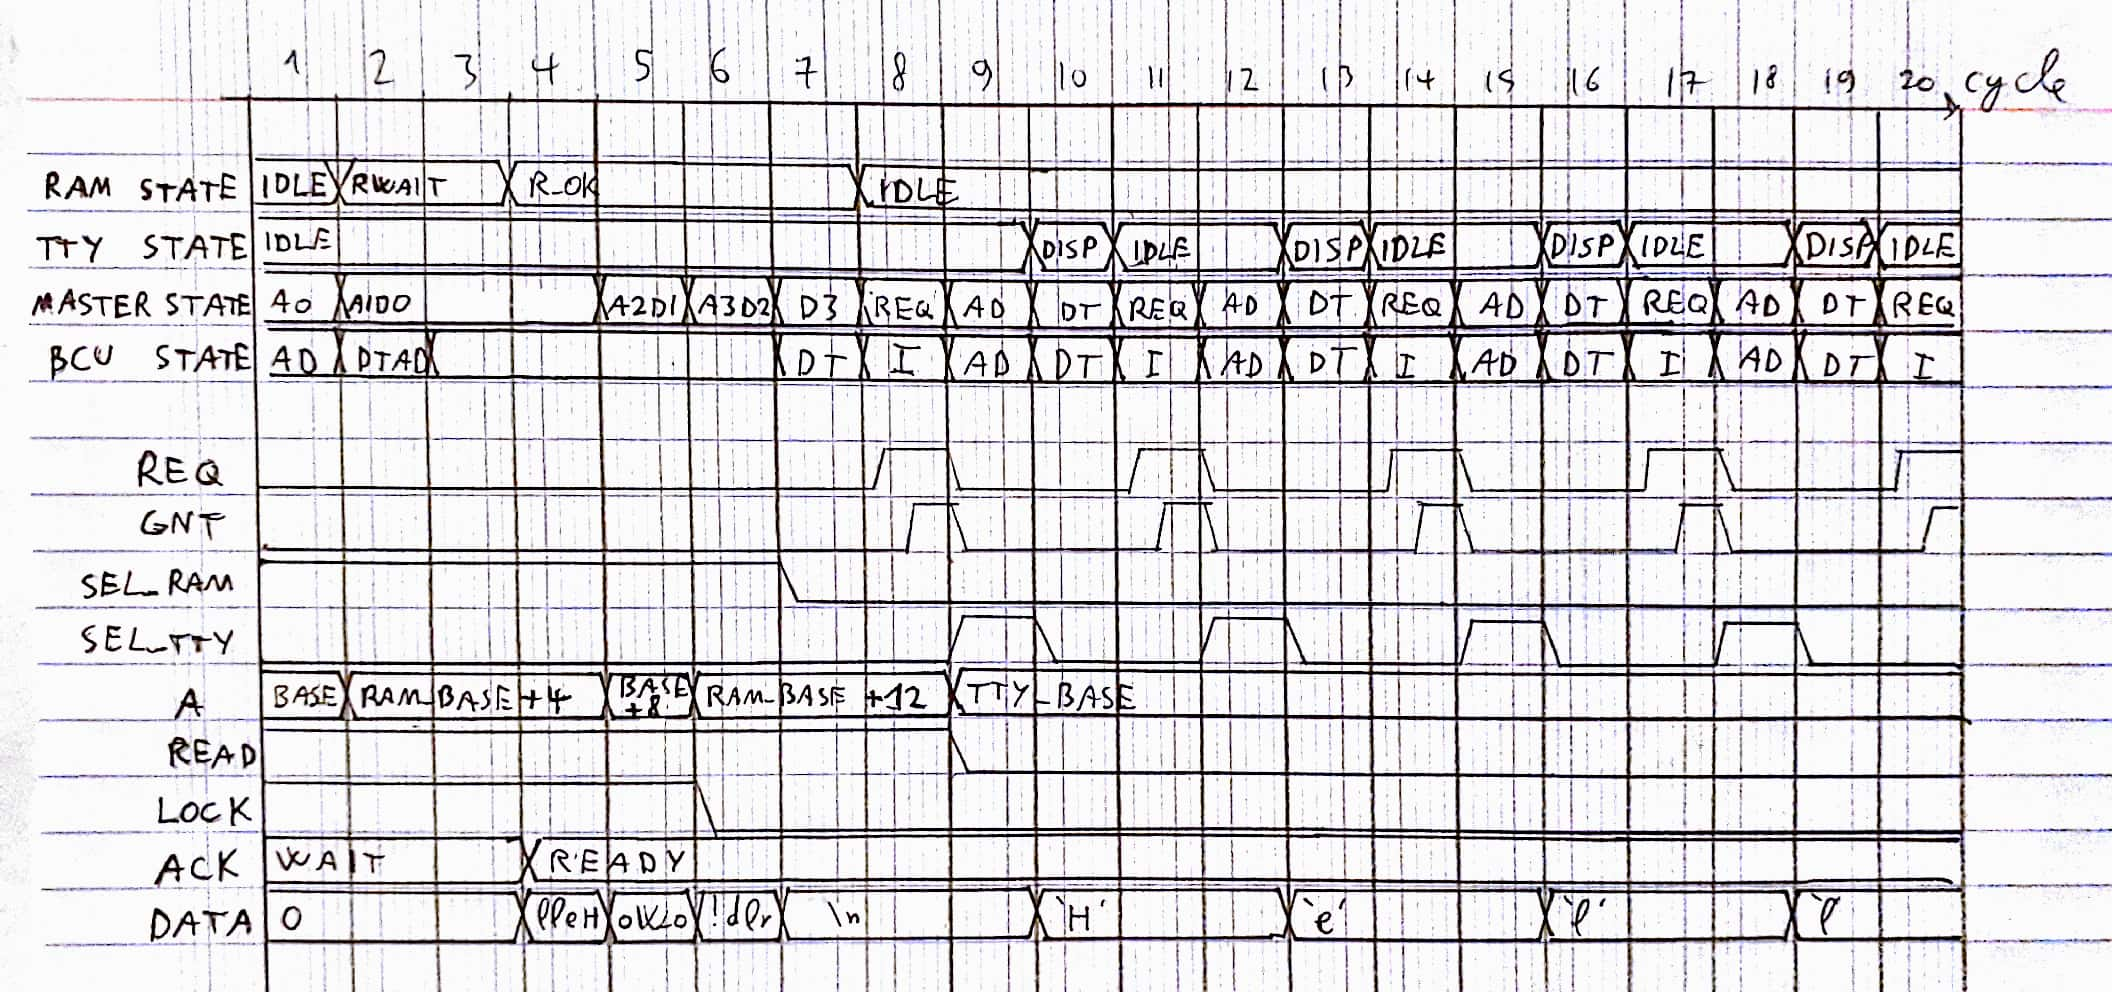
\includegraphics[width=\textwidth]{pics/chrono.png}
\centering
\caption{Chronogramme des signaux du PIBUS}
\label{mae_ram}
\end{figure}






%==================================================================================================
%=========================  End of the Document  ==================================================
%==================================================================================================

\end{document}
